
\section{Simulation of the MPPT} \label{MPPTSimulation}

The results obtained in simulation for the previously explained P\&O algorithm will be shown in this section. First, the results corresponding to the PV panel model will be evaluated without connecting it to the DC-DC converter. Once the model for the PV panel is validated, the results obtained for the complete system will be analyzed in order to show the performance of the MPPT algorithm under different environmental conditions and resistive loads.  

\subsection{Model of the PV panel}

This section shows the model and the results obtained from a commercial solar panel selected for the development of this project. The PV panel which will be utilized for the test of the MPPT is \textit{Suntech STP300-24/Vd} \cite{PV_panel}. As a result of the PV panel's model, the characteristic curves of the panel will be presented showing its behavior under variations in solar irradiance and temperature.

One of the most common methods for modeling a solar panel is using the equivalent circuit of a solar cell shown in figure \ref{fig:eq_circuit_PVcell}. The model can be represented as a current source connected in antiparallel with a diode \cite{MPPTResearch}. In addition, to model the non-linear behaviour of the solar panel I-V curve the equivalent series and parallel resistance ($R_{s}$ and $R_{p}$) are inserted \cite{MPPTResearch}.

\begin{figure}[H]
	\begin{center}
		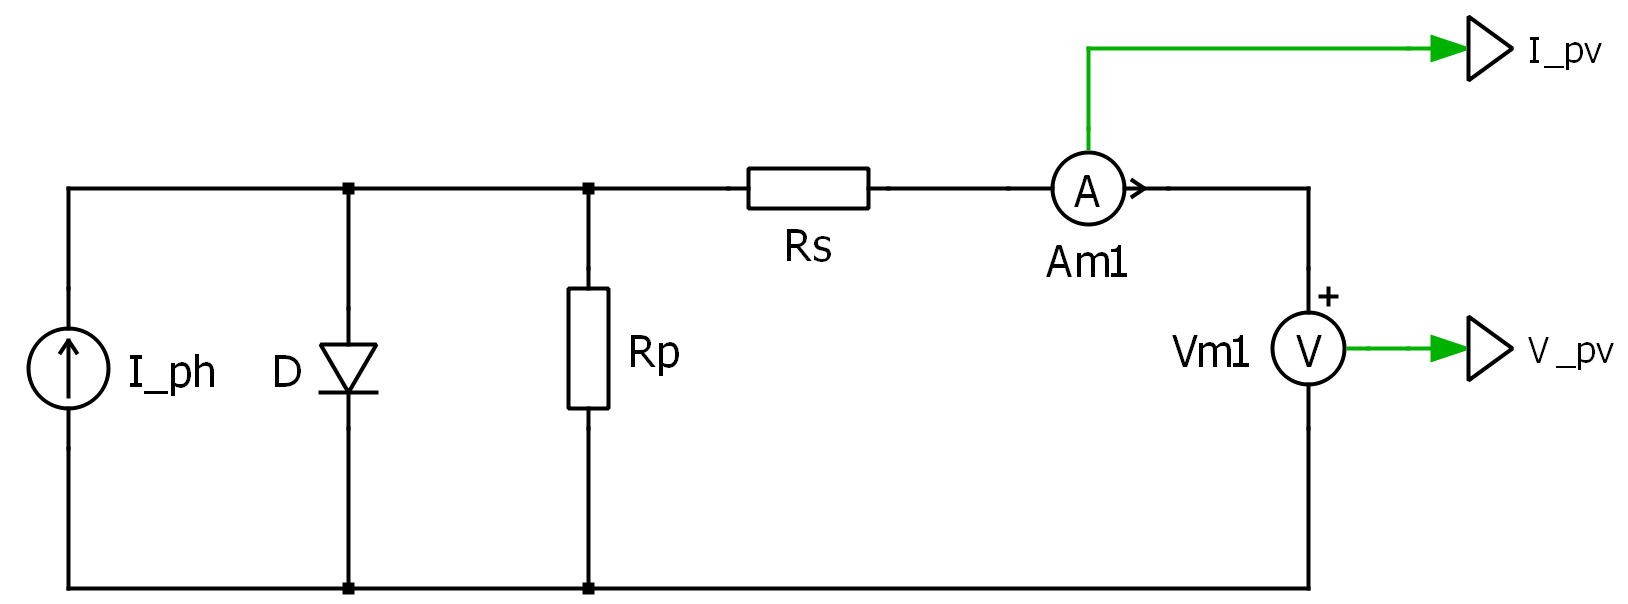
\includegraphics[width=0.75\textwidth]{../Pictures/schematic_solar_cell}
		\caption{Equivalent circuit for modeling a PV cell.}
		\label{fig:eq_circuit_PVcell} 
	\end{center}	
\end{figure}

The mathematical equation that describes the circuit is obtained applying Kirchoff's law to separate the current flowing through the different components of the circuit. This results in equation \ref{eq:pv_cell} where $I_{pv}$ is the panel's current, $I_{ph}$ is the photogenerated current, the second term is the current flow in the diode and the last term is the current flow in the parallel resistance \cite{MPPTResearch}. 

\begin{equation} \label{eq:pv_cell}
I_{pv} = I_{ph} - I_{o} \cdot \left[ e^{\left({\dfrac{V_{pv} + R_s\cdot I_{pv}}{a \cdot V_{t}}}\right)}  - 1 \right]  - \dfrac{V_{pv} + R_{s}\cdot I_{pv}}{R_{p}}
\end{equation}

The second term corresponds to the Shockley equation where $I_{o}$ is the saturation current of the diode, $a$ is the diode's quality factor and $V_{t}$ is the thermal voltage defined by

\begin{equation} 
V_{t}=\dfrac{N_{s}\cdot K\cdot T}{q} 
\end{equation}

where $N_{s}$ is the number of series connected cells (in this case 72), K is the Boltzmann constant ($1.38 \cdot 10^{-23} J/K$), T is the temperature in kelvins and q is the electrical charge ($1.6 \cdot 10^{-19} C$) \cite{MPPTResearch}.

However, as the focus of this project is not the modelling of the PV panel, the value of the PV panel's parameters such as $R_{s}$, $R_{p}$ and $a$ required for the model will not be calculated. Instead, these values will be taken from the corresponding PV array block for the selected panel available in \textit{Simulink}. All the values for the PV panel's electrical parameters corresponding to Standard Test Conditions (STC) are shown in table \ref{el_charact_PV_panel_Suntech}.

\begin{table}[H]
	\centering
	\begin{tabular}{|p{8cm}|>{\centering}p{6cm}|}
		\hline
		\rowcolor{lightgray}\multicolumn{2}{|l|}{ \textbf{Electrical characteristics under Standard Test Conditions (STC)}} 
		\\ \hline
		Maximum power ($P_{max}$) & 300 [W]  \tabularnewline \hline
		Optimum Operating Voltage ($V_{mpp}$) & 36.9 [V]  \tabularnewline \hline
		Optimum Operating Current ($I_{mpp}$) & 8.14 [A]  \tabularnewline \hline
		Open Circuit Voltage ($V_{oc}$) &  45 [V] \tabularnewline \hline
		Short Circuit Current ($I_{sc}$) & 8.67 [A]  \tabularnewline \hline
		Module Efficiency ($\eta$) & 15.5 \%  \tabularnewline \hline
		Operating Module Temperature & -40$\dec$C to +85$\dec$C \tabularnewline \hline
		Series Resistance ($R_{s}$) & 0.266 [$\Omega$] \tabularnewline \hline
		Parallel Resistance ($R_{p}$) & 665.2 [$\Omega$] \tabularnewline \hline
		Diode quality factor ($a$) & 1.1098 \tabularnewline \hline
	\end{tabular}
	\caption{Electrical characteristics PV module \textit{Suntech STP300-24/Vd} \cite{PV_panel}.}
	\label{el_charact_PV_panel_Suntech}
\end{table}

Using the aforementioned model of the PV panel, it is possible to obtain the characteristic curves of the panel.  Usually, PV panels are tested under STC to indicate the performance of the PV modules. The STC test is carried out at a solar cell's temperature of $25^\circ$C and at a solar irradiance of 1000 $W/ m^2$ \cite{handbook}. The higher the solar irradiance more power is generated from the PV panel. On the other hand, when the temperature of the PV cell increases the PV panel generates less power than at a lower temperature \cite{handbook}. 

Figures \ref{fig:PVcurves_T25} and \ref{fig:IVcurves_T25} show the P-V and I-V curves of the solar panel with constant cell temperature ($T=25\dec C$) and varying the level of irradiance. 
As expected, the lower the level of irradiance the maximum power that the panel is capable of generating decreases. It can be validated that under STC the values for $V_{mpp}$ and $I_{mpp}$ from table \ref{el_charact_PV_panel_Suntech}  correspond to the values obtained in simulation. Table \ref{constantemptable} shows that a change in irradiance has as a consequence a high variation in $I_{mpp}$ but $V_{mpp}$ does not reflect a significant variation.  


\begin{figure}[H]
	\begin{center}
		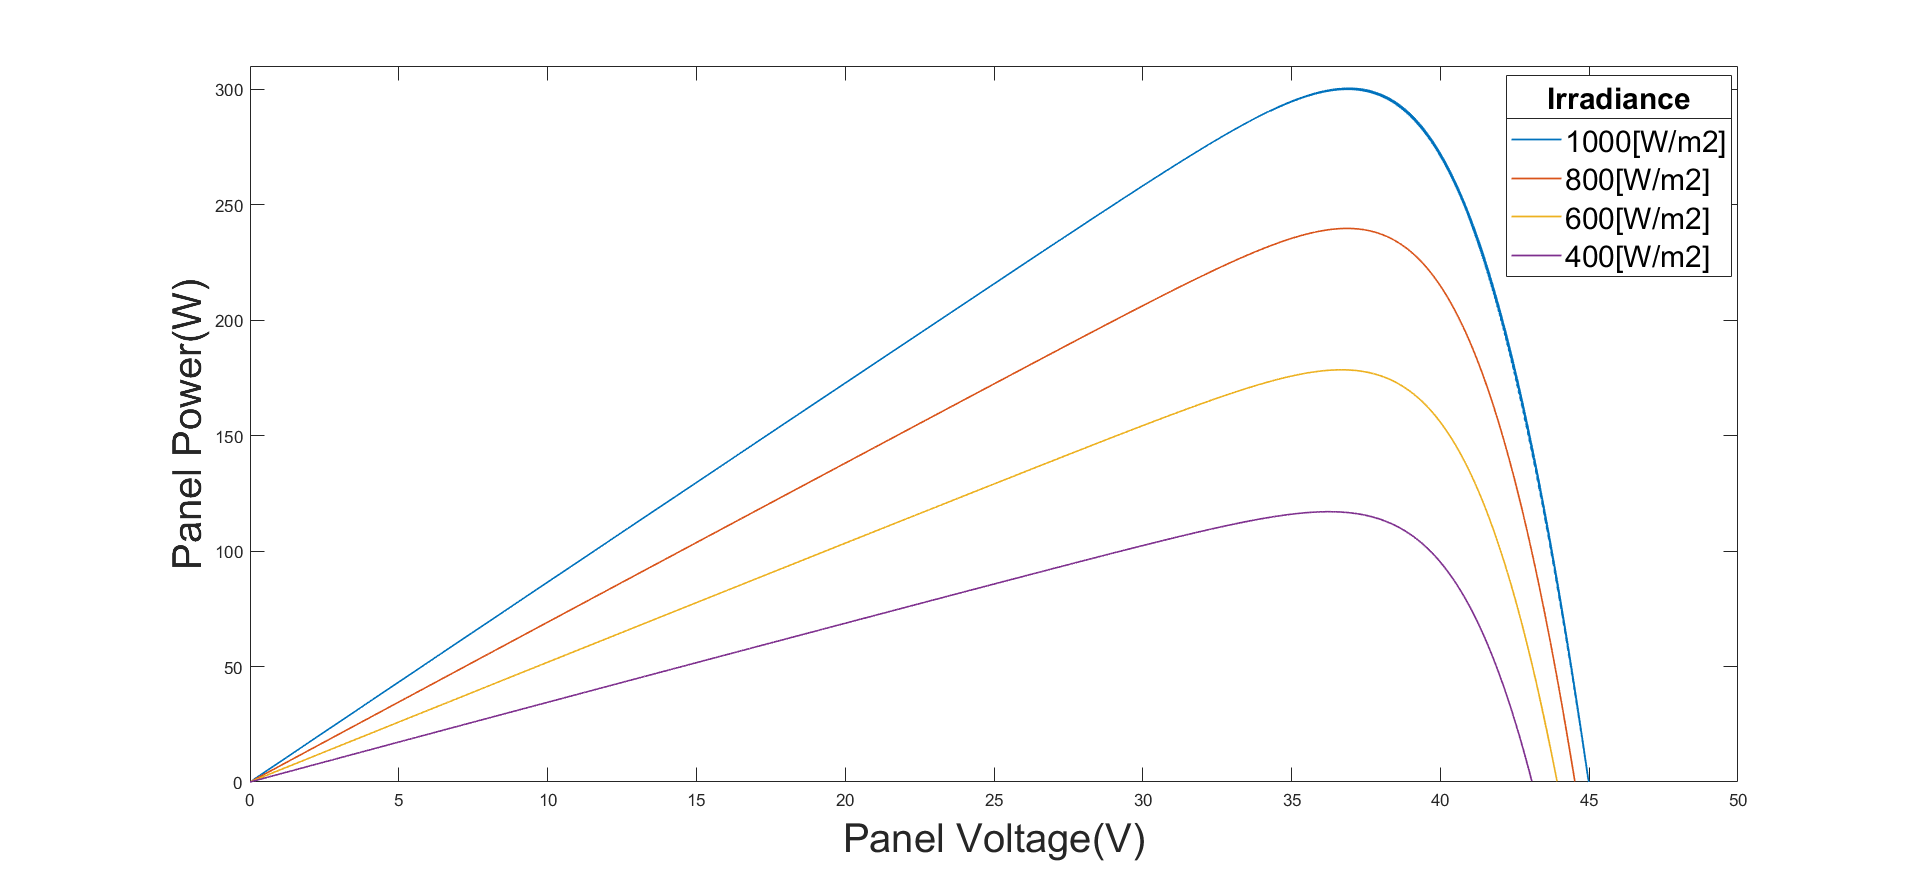
\includegraphics[width=0.97\textwidth]{../Pictures/constant_temperature}
		\caption{P-V curves for constant temperature (25$\dec$C) and change in irradiance.}
		\label{fig:PVcurves_T25} 
	\end{center}	
\end{figure}

\begin{figure}[H]
	\begin{center}
		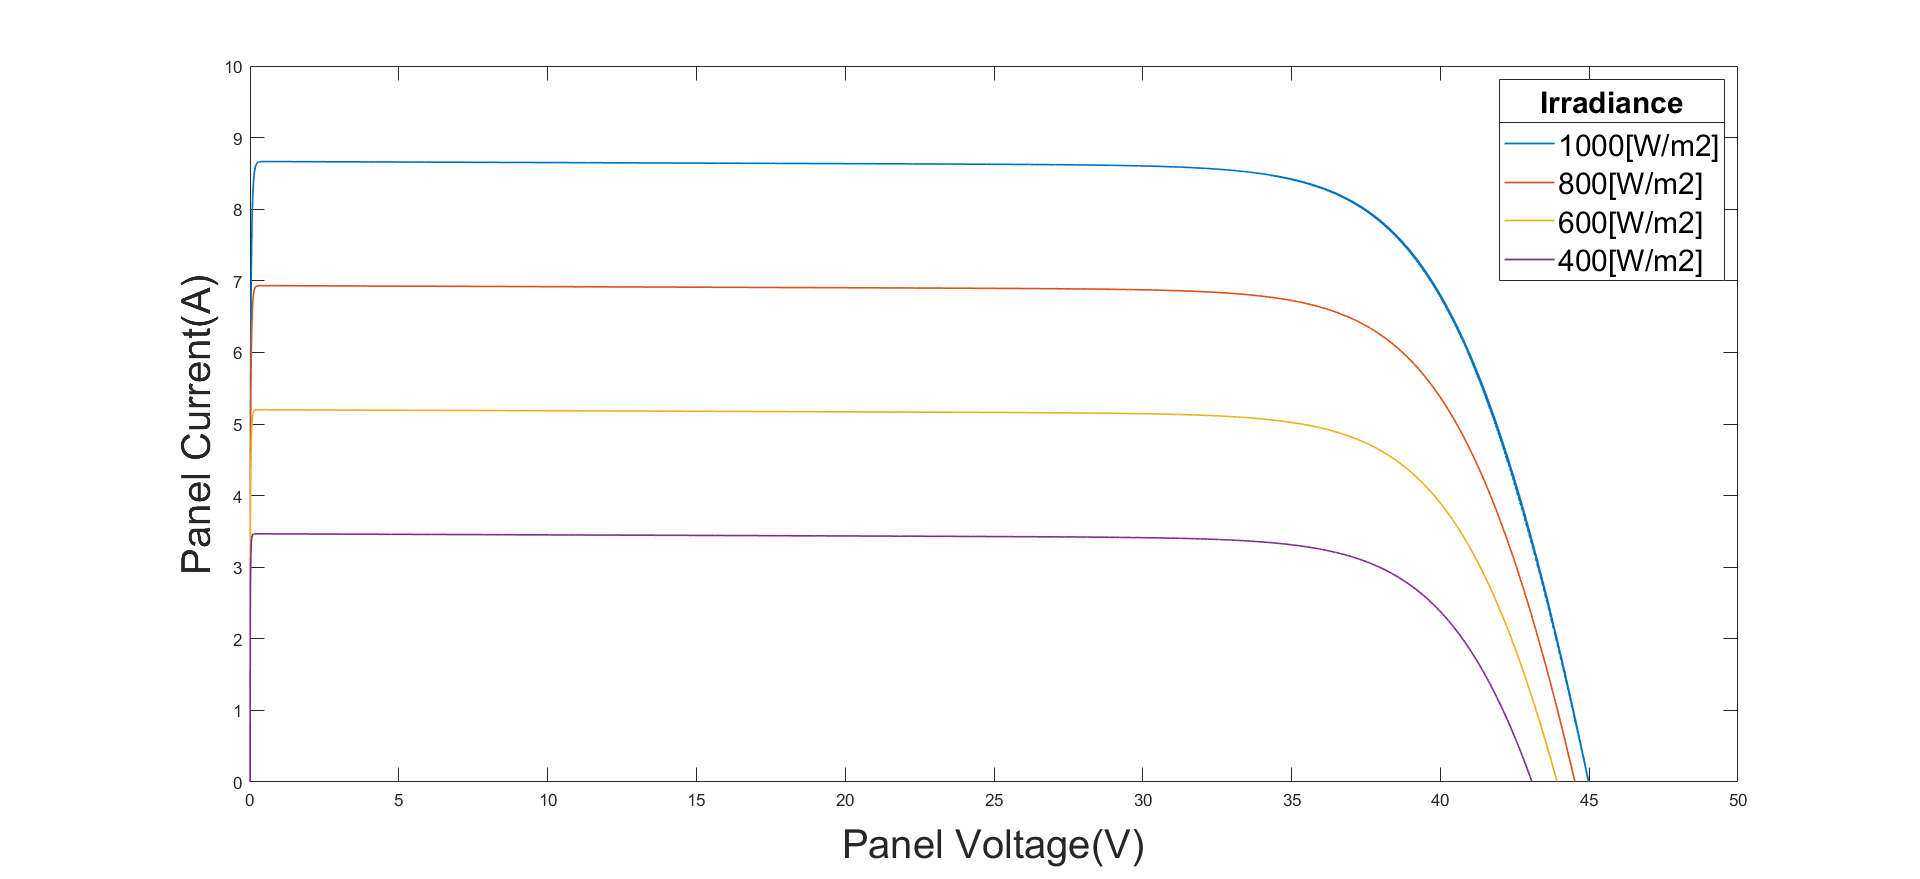
\includegraphics[width=0.97\textwidth]{../Pictures/constant_temperature_iv}
		\caption{I-V curves for constant temperature (25$\dec$C) and change in irradiance.}
		\label{fig:IVcurves_T25} 
	\end{center}	
\end{figure}


\begin{table}[H]
	\centering
	\begin{tabular}{|p{2cm}|>{\centering}p{2cm}|>{\centering}p{2cm}|>{\centering}p{2cm}|>{\centering}p{2cm}|}
		\hline
		\rowcolor{lightgray}\multicolumn{5}{|l|}{ \textbf{Constant temperature 25$\dec$C and varying irradiance}} 
		\\ \hline
		& 1000$W/ m^2$ & 800$W/ m^2$  & 600$W/ m^2$  & 400$W/ m^2$ \tabularnewline \hline
		$V_{mpp}$ [V] & 36.9 & 36.87 & 36.68 & 36.19 \tabularnewline \hline
		$I_{mpp}$ [A] & 8.14 & 6.49 & 4.86 & 3.23 \tabularnewline \hline
		$P_{mpp}$ [W] &  300.4 &  239.5 &  178.5 &  117 \tabularnewline \hline
	\end{tabular}
	\caption{Results of the optimum PV panel parameters for varying irradiance.}
	\label{constantemptable}
\end{table}

On the other hand, figures \ref{fig:PVcurves_Irr1000} and \ref{fig:IVcurves_Irr1000} show the characteristic curves with constant irradiance (1000$W/ m^2$) and under temperature variation.

\begin{figure}[H]
	\begin{center}
		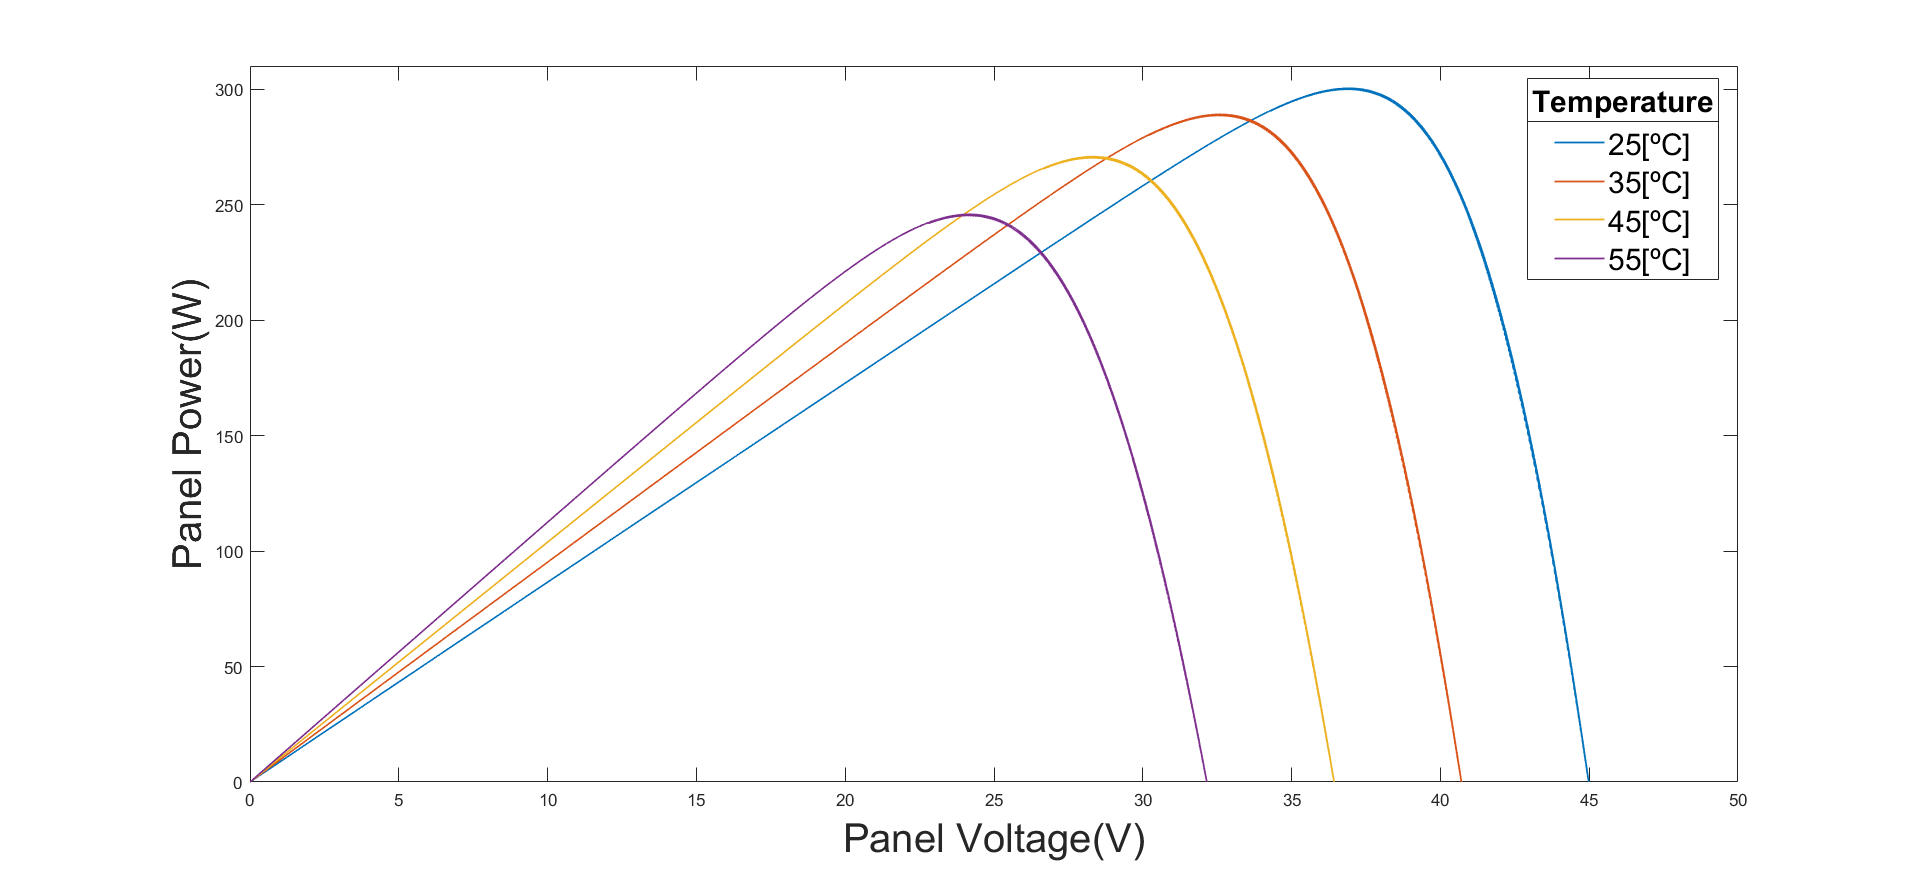
\includegraphics[width=0.96\textwidth]{../Pictures/constant_irradiance}
		\caption{P-V curves for constant irradiance (1000$W/ m^2$) and change in temperature.}
		\label{fig:PVcurves_Irr1000} 
	\end{center}	
\end{figure}


\begin{figure}[H]
	\begin{center}
		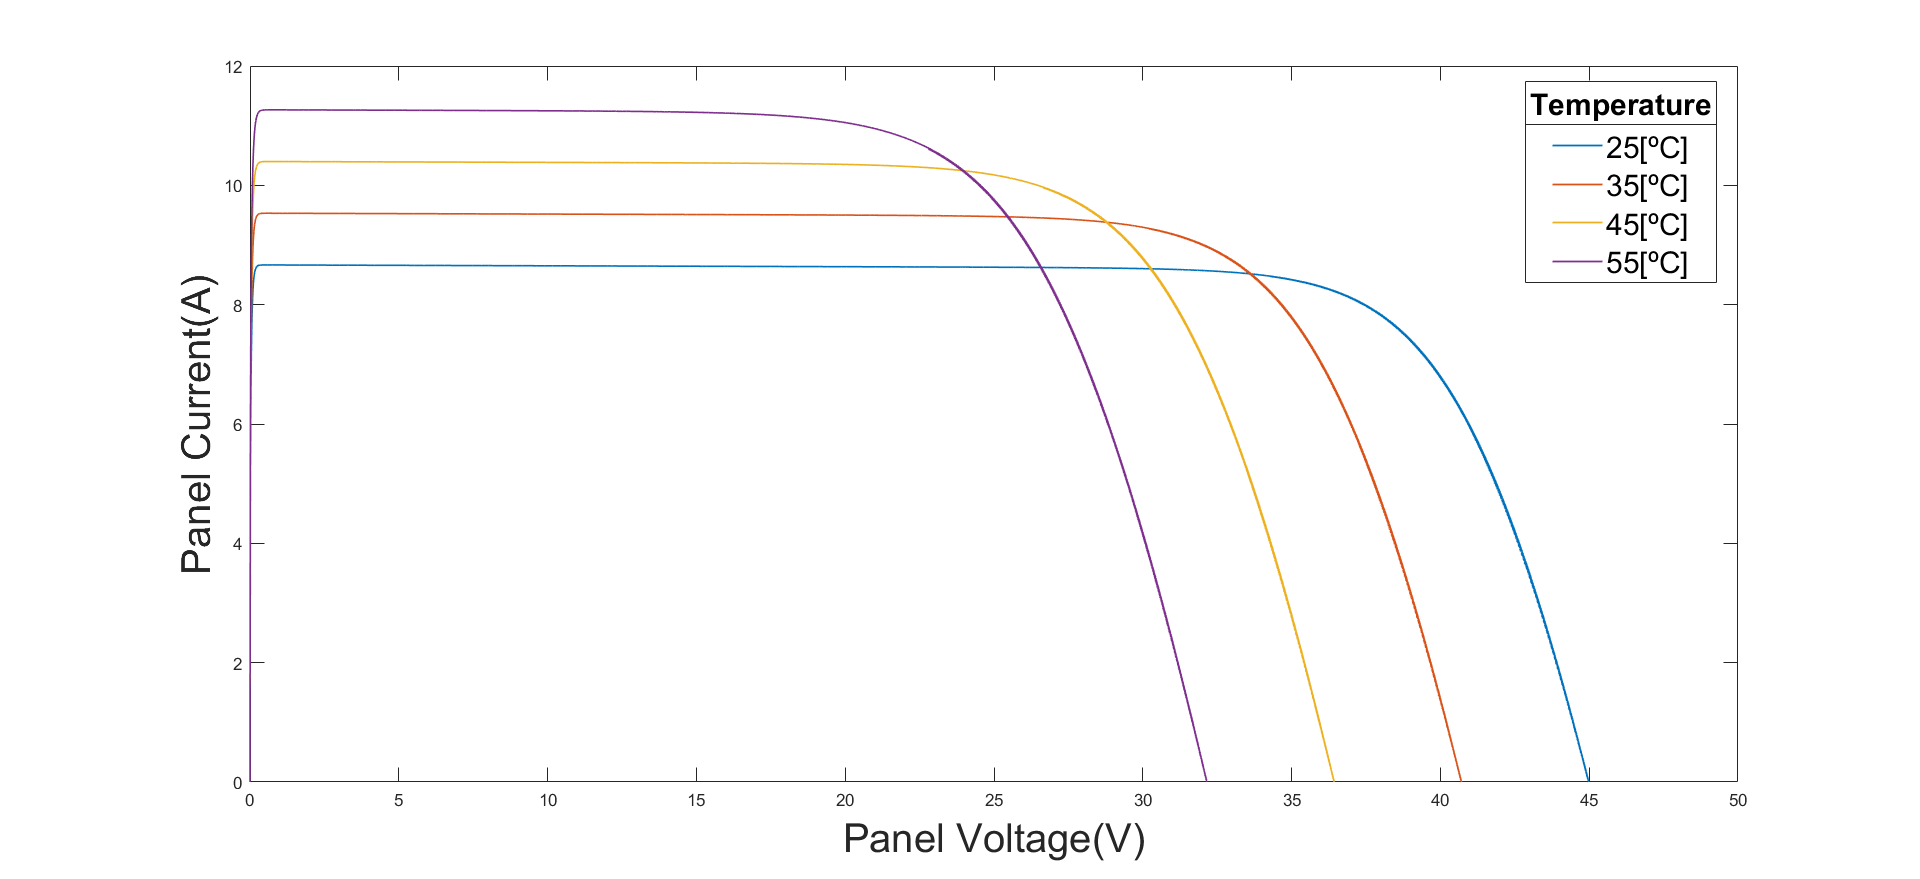
\includegraphics[width=0.96\textwidth]{../Pictures/iv_constant_irradiance}
		\caption{I-V curves for constant irradiance (1000$W/ m^2$) and change in temperature.}
		\label{fig:IVcurves_Irr1000} 
	\end{center}	
\end{figure}

 It is observed from table \ref{constantirradtable} that an increase in the temperature means that the maximum power that the panel is able to generate decreases. In this case, a change in temperature has as a consequence a high variation of $V_{mpp}$. However, the variation is not that significant in $I_{mpp}$.
 

\begin{table}[H]
	\centering
	\begin{tabular}{|p{2cm}|>{\centering}p{2cm}|>{\centering}p{2cm}|>{\centering}p{2cm}|>{\centering}p{2cm}|}
		\hline
		\rowcolor{lightgray}\multicolumn{5}{|l|}{ \textbf{Constant irradiance 1000$W/ m^2$ and varying temperature}} 
		\\ \hline
		& T=25$\dec C$  & T=35$\dec C$  & T=45$\dec C$  & T=55$\dec C$ \tabularnewline \hline
		$V_{mpp}$ [V] & 36.9 & 32.59 & 28.34 & 24.23\tabularnewline \hline
		$I_{mpp}$ [A] & 8.14 & 8.85 & 9.59 & 10.12 \tabularnewline \hline
		$P_{mpp}$ [W] &  300.4 &  289.1 &  270.7 &  245.8 \tabularnewline \hline
	\end{tabular}
	\caption{Results of the optimum PV panel parameters for varying temperature.}
	\label{constantirradtable}
\end{table}

\subsection{Simulation results}

\iffalse
\begin{figure}[H]
	\begin{minipage}[c]{0.6\textwidth}
		\centering
		\includegraphics[width=1\textwidth]{../Pictures/P1/simulationMPPT/V_I_P_buck(R=3)_STC} % Left picture
	\end{minipage}%
	\hfill
	\begin{minipage}[c]{0.6\textwidth}
		\centering
		\includegraphics[width=1\textwidth]{../Pictures/P1/simulationMPPT/V_I_P_boost(R=27)_STC} % Right picture
	\end{minipage} \\ % Captions og labels
	\begin{minipage}[t]{0.6\textwidth}
		\caption{buck STC V,I,P.} % Left caption and label
		\label{buckSTC}
	\end{minipage}%
	\hfill
	\begin{minipage}[t]{0.6\textwidth}
		\caption{boost STC V,I,P} % Right caption and label
		\label{boostSTC}
	\end{minipage}
\end{figure}

\begin{figure}[H]
	\begin{minipage}[c]{0.6\textwidth}
		\centering
		\includegraphics[width=1\textwidth]{../Pictures/P1/simulationMPPT/Dutys_Vpv_Vout_buck(R=3)_STC} % Left picture
	\end{minipage}%
	\hfill
	\begin{minipage}[c]{0.6\textwidth}
		\centering
		\includegraphics[width=1\textwidth]{../Pictures/P1/simulationMPPT/Dutys_Vpv_Vout_boost(R=27)_STC} % Right picture
	\end{minipage} \\ % Captions og labels
	\begin{minipage}[t]{0.6\textwidth}
		\caption{buck STC duty vin vs vout} % Left caption and label
		\label{buckSTC_duty}
	\end{minipage}%
	\hfill
	\begin{minipage}[t]{0.6\textwidth}
		\caption{boost STC duty vin vs vout} % Right caption and label
		\label{boostSTC_duty}
	\end{minipage}
\end{figure}
\fi 

In this section, the results obtained in simulation for the entire system will be presented. The system includes the solar panel, the non-inverting buck-boost converter and the MPPT controller unit as shown in figure \ref{BD_POalgorithm}. The simulated results will be analyzed to determine the performance of the MPPT and will be divided in two parts: 
\begin{itemize}
	\item[--] Results obtained under STC. The STC test is carried out at a solar cell's temperature of $25^\circ$C and at a solar irradiance of 1000 $W/ m^2$ \cite{handbook}.
	\item[--] Results obtained under a sudden change in the solar irradiance and temperature.
\end{itemize}

 It was decided to use a resistive load to validate the results obtained in the simulation with the experimental results. All the simulations will be carried out for two different resistive loads: $R_{L}=3\Omega$ and $R_{L}=27\Omega$. This is done in order to validate the performance of the MPPT controller in both modes of operation.
 \subsubsection*{Standard Test Conditions (STC)}
 
 Figure \ref{buckSTC} shows how the P\&O algorithm searchs for the MPP. The first graph shows a superposition of the PV panel's voltage and current where it is observed that the panel reaches the open-circuit voltage ($V_{oc}=45 V$) and at that moment the MPPT starts searching for the MPP by decreasing the PV voltage. The second graph shows the power generated by the panel which approaches the value of the optimal power under this conditions ($P_{mpp}=300 W$). The P\&O algorithm converges to the MPP reaching the steady state in 2 seconds. The MPPT allows to reach the optimal power generated by the panel under this conditions with an efficiency of $\eta_{MPPT} = 99.96\% $.
\begin{figure}[H]
	\begin{center}
		\includegraphics[width=0.8\textwidth]{../Pictures/P1/simulationMPPT/V_I_P_buck(R=3)_STC}
		\caption{Voltage, current and power extracted from the PV panel ($R_{L}=3\Omega$).}
		\label{buckSTC} 
	\end{center}	
\end{figure}

The simulation is run under STC and using a resistive load of $3\Omega$. From the first graph of figure \ref{buckSTC_duty} it is observed that the converter is working in buck mode during all the MPPT process. This is because the output voltage does not exceeds the input voltage with this resistive load as shown in the second graph. The value of the duty cycle, obtained in simulation under these load and environment conditions, is $D_{buck}= 0.8155$. Using the transfer function of the converter in  buck mode, this value can be validated by calculating the theoretical duty cycle taking as voltage input $V_{mpp}=36.9 V$: 

\begin{equation}\label{buckmodeTF}
\frac{V_{out}}{V_{in}} = D  \rightarrow D = \frac{30V}{36.9V}= 0.8130 
\end{equation}


\begin{figure}[H]
	\begin{center}
		\includegraphics[width=0.8\textwidth]{../Pictures/P1/simulationMPPT/Dutys_Vpv_Vout_buck(R=3)_STC}
		\caption{Converter's mode of operation as a function of the control variable ($R_{L}=3\Omega$).}
		\label{buckSTC_duty} 
	\end{center}	
\end{figure}

The same simulation was implemented but in this case using a value of the resistive load of $27\Omega$. From figure \ref{boostSTC} it is observed that the MPPT needs more time than before to converge to the MPP. The P\&O algorithm needs 4 seconds to reach the MPP which means double of the time than with $R_{L}=3\Omega$. This occurs because the output voltage starts increasing from 0 to its final value. This means that the system will start working in buck mode and once the output voltage reaches the value of the input voltage it will switch to boost mode. Despite the higher converging time to the MPP, the P\&O algorithm performance has not experience a significant difference. The MPPT is able to operate with an efficiency of $\eta_{MPPT} = 99.82\% $.


\begin{figure}[H]
	\begin{center}
		\includegraphics[width=0.8\textwidth]{../Pictures/P1/simulationMPPT/V_I_P_boost(R=27)_STC}
		\caption{Voltage, current and power extracted from the PV panel ($R_{L}=27\Omega$).}
		\label{boostSTC} 
	\end{center}	
\end{figure}

Figure \ref{boostSTC_duty} shows how the converter starts operating in buck mode until the output voltage equals the input voltage. At this point is the limit between the two modes of operation and the converter starts working in boost mode. The value of the duty cycle under these load and environment conditions is $D_{boost}= 0.5971$. sing the transfer function of the converter in  buck mode, this value can be validated by calculating the theoretical duty cycle taking as voltage input $V_{mpp}=36.9 V$: 
\begin{equation}
\frac{V_{out}}{V_{in}}= \frac{1}{1-D} \rightarrow D = 1 - \frac{V_{in}}{V_{out}} = 1 - \frac{36.9}{90} = 0.5900
\end{equation}
 
\begin{figure}[H]
	\begin{center}
		\includegraphics[width=0.8\textwidth]{../Pictures/P1/simulationMPPT/Dutys_Vpv_Vout_boost(R=27)_STC}
		\caption{Converter's mode of operation as a function of the control variable ($R_{L}=27\Omega$).}
		\label{boostSTC_duty} 
	\end{center}	
\end{figure}

\subsubsection*{Change in irradiance and temperature}

This section shows the performance of the MPPT when the PV panel is exposed to a sudden change in irradiance and in temperature. First, figures \ref{buckirradiance} and \ref{boostirradiance} show the results obtained for a change in irradiance for the case of buck and boost mode, respectively. The irradiance change is from 1000 $W/ m^2$ to 800 $W/ m^2$ while the cell temperature is kept constant at 25 $\dec$C. 
Figures \ref{bucktemperature} and \ref{boosttemperature}  show the results for a sudden increase of the solar cell's temperature for both modes of operation. The temperature changes from 25 $\dec$C to 35 $\dec$C by keeping constant the irradiance to a value of 1000 $W/ m^2$. 
In all the cases the P\&O algorithm can track the MPP by maintaining an efficiency higher than 99\%. This way it is validated that the MPPT algorithm works efficiently under sudden changes of irradiance and temperature. However, this situations are not realistic because in real environmental conditions the sunlight and the temperature will not experience such a sudden change. 

\begin{figure}[H]
	\begin{minipage}[c]{0.6\textwidth}
		\centering
		\includegraphics[width=1\textwidth]{../Pictures/P1/simulationMPPT/V_I_P_buck(R=3)_irradiance_1000_800} % Left picture
	\end{minipage}%
	\hfill
	\begin{minipage}[c]{0.6\textwidth}
		\centering
		\includegraphics[width=1\textwidth]{../Pictures/P1/simulationMPPT/V_I_P_boost(R=27)_irradiance_1000_800} % Right picture
	\end{minipage} \\ % Captions og labels
	\begin{minipage}[t]{0.6\textwidth}
		\caption{Irradiance 1000-800$W/ m^2$ ($R_{L}=3\Omega$).} % Left caption and label
		\label{buckirradiance}
	\end{minipage}%
	\hfill
	\begin{minipage}[t]{0.6\textwidth}
		\caption{Irradiance 1000-800$W/ m^2$ ($R_{L}=27\Omega$).} % Right caption and label
		\label{boostirradiance}
	\end{minipage}
\end{figure}

\iffalse
\begin{figure}[H]
	\begin{center}
		\includegraphics[width=0.8\textwidth]{../Pictures/P1/simulationMPPT/V_I_P_buck(R=3)_irradiance_1000_800}
		\caption{buck change irradiance V,I,P}
		\label{buckirradiance} 
	\end{center}	
\end{figure}


\begin{figure}[H]
	\begin{center}
		\includegraphics[width=0.8\textwidth]{../Pictures/P1/simulationMPPT/V_I_P_boost(R=27)_irradiance_1000_800}
		\caption{boost change irradiance V,I,P}
		\label{boostirradiance} 
	\end{center}	
\end{figure}
\fi

\vspace{1cm}
\begin{figure}[H]
	\begin{minipage}[c]{0.6\textwidth}
		\centering
		\includegraphics[width=1\textwidth]{../Pictures/P1/simulationMPPT/V_I_P_buck(R=3)_temperature_25_45} % Left picture
	\end{minipage}%
	\hfill
	\begin{minipage}[c]{0.6\textwidth}
		\centering
		\includegraphics[width=1\textwidth]{../Pictures/P1/simulationMPPT/V_I_P_boost(R=27)_temperature_25_45} % Right picture
	\end{minipage} \\ % Captions og labels
	\begin{minipage}[t]{0.6\textwidth}
		\caption{Temperature 25-35$\dec C$ ($R_{L}=3\Omega$).} % Left caption and label
		\label{bucktemperature}
	\end{minipage}%
	\hfill
	\begin{minipage}[t]{0.6\textwidth}
		\caption{Temperature 25-35$\dec C$ ($R_{L}=27\Omega$).} % Right caption and label
		\label{boosttemperature}
	\end{minipage}
\end{figure}

\iffalse
\begin{figure}[H]
	\begin{center}
		\includegraphics[width=0.8\textwidth]{../Pictures/P1/simulationMPPT/V_I_P_buck(R=3)_temperature_25_45}
		\caption{buck change T V,I,P}
		\label{bucktemperature} 
	\end{center}	
\end{figure}

\begin{figure}[H]
	\begin{center}
		\includegraphics[width=0.8\textwidth]{../Pictures/P1/simulationMPPT/V_I_P_boost(R=27)_temperature_25_45}
		\caption{boost change T V,I,P}
		\label{boostirradiance} 
	\end{center}	
\end{figure}
\fi